\documentclass[11pt]{article}
\usepackage{minted, tikz}
\usepackage{amsfonts, amssymb, amsmath, float, tabularx}
\usepackage{enumerate, esint, nicefrac, algorithm2e}
\parindent 0px
\date{October 18, 2023}
\title{CS301 :: Homework 3}
\author{Ryan Magdaleno}
\begin{document}
\maketitle

%%%%%%%%%%%%%%%%%%%%%%%%%%%%%%%%%%%%%%%%%%%%%%%%%%%%%%%%%%%%%%%%%%%%%%%%%%%%%%%%%%%%%%%%%

\textbf{Problem 1. Regular Grammars} 

Consider the following language $L.$ $\sum = \{0, 1\}$. \textbf{You do not need to
produce any tuples.}
$$L = \{w : w\text{ has an even number of 0s and an odd number of 1s}\}$$
\begin{enumerate}[a)]
\item 
Give the NFA which decides L.

\vspace{5px}\textbf{Solution ::}
\begin{center}
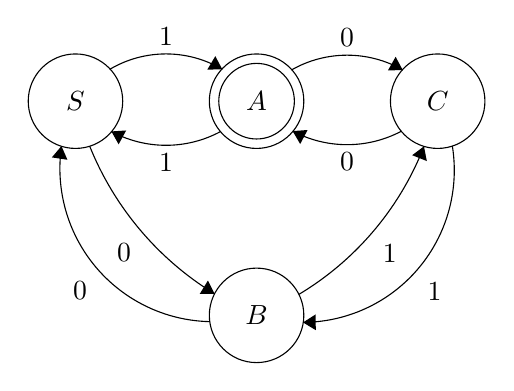
\begin{tikzpicture}[scale=0.2]
\tikzstyle{every node}+=[inner sep=0pt]
\draw [black] (18.2,-17.8) circle (3);
\draw (18.2,-17.8) node {$S$};
\draw [black] (29.7,-17.8) circle (3);
\draw (29.7,-17.8) node {$A$};
\draw [black] (29.7,-17.8) circle (2.4);
\draw [black] (41.2,-17.8) circle (3);
\draw (41.2,-17.8) node {$C$};
\draw [black] (29.7,-31.4) circle (3);
\draw (29.7,-31.4) node {$B$};
\draw [black] (20.382,-15.775) arc (120.60442:59.39558:7.008);
\fill [black] (27.52,-15.77) -- (27.08,-14.94) -- (26.57,-15.8);
\draw (23.95,-14.3) node [above] {$1$};
\draw [black] (27.424,-19.722) arc (-61.58828:-118.41172:7.302);
\fill [black] (20.48,-19.72) -- (20.94,-20.54) -- (21.42,-19.66);
\draw (23.95,-21.1) node [below] {$1$};
\draw [black] (31.92,-15.815) arc (119.72251:60.27749:7.12);
\fill [black] (38.98,-15.82) -- (38.53,-14.98) -- (38.04,-15.85);
\draw (35.45,-14.38) node [above] {$0$};
\draw [black] (38.906,-19.701) arc (-62.02541:-117.97459:7.367);
\fill [black] (31.99,-19.7) -- (32.47,-20.52) -- (32.94,-19.63);
\draw (35.45,-21.06) node [below] {$0$};
\draw [black] (42.13,-20.64) arc (9.23101:-89.66594:9.657);
\fill [black] (32.65,-31.85) -- (33.46,-32.34) -- (33.45,-31.34);
\draw (40.52,-29.86) node [right] {$1$};
\draw [black] (40.333,-20.669) arc (-21.34322:-59.09171:19.026);
\fill [black] (40.33,-20.67) -- (39.58,-21.23) -- (40.51,-21.6);
\draw (37.69,-27.47) node [right] {$1$};
\draw [black] (26.739,-31.799) arc (-91.157:-188.40806:9.725);
\fill [black] (17.31,-20.65) -- (16.7,-21.37) -- (17.69,-21.52);
\draw (18.96,-29.8) node [left] {$0$};
\draw [black] (27.032,-30.034) arc (-121.50747:-158.0576:19.579);
\fill [black] (27.03,-30.03) -- (26.61,-29.19) -- (26.09,-30.04);
\draw (21.76,-27.42) node [left] {$0$};
\end{tikzpicture}
\end{center}
\line(1,0){343px}
\item
Produce the right-linear, single-step CFG which is equivalent to your NFA in a).

\vspace{5px}\textbf{Solution ::}
\begin{align}
    S&\longrightarrow 1A \,|\, 0B \\
    A&\longrightarrow 1S\,|\, OC \,|\, \epsilon \\
    B&\longrightarrow 0S \,|\, 1C \\
    C&\longrightarrow 0A \,|\, 1B
\end{align}
\end{enumerate}

\pagebreak

%%%%%%%%%%%%%%%%%%%%%%%%%%%%%%%%%%%%%%%%%%%%%%%%%%%%%%%%%%%%%%%%%%%%%%%%%%%%%%%%%%%%%%%%%

\textbf{Problem 2. Context Free Grammars}

Produce the CFG for the following languages. $\sum = \{a,b,c\}$. \textit{You do not need
to produce the 4-tuples.}
\begin{enumerate}[a)]
\item 
$L_a = \{w \text{ : the \# of a's is equal to the \# of b's and c's combined\,}\}$

\vspace{5px}\textbf{Solution ::}
\begin{align}
    S&\longrightarrow aSx \,|\, xSa \,|\, SaX \,|\, XaS \,|\, SXa \,|\, XSa \\
    S&\longrightarrow \epsilon \\
    X&\longrightarrow b \,|\, c
\end{align}
\line(1,0){343px}

\item 
$L_b=\{a^ib^{2j}c^{i+j} : i, j \ge 1\}$

\vspace{5px}\textbf{Solution ::}
\begin{align}
    S&\longrightarrow aSc \,|\, abbXcc \\
    X&\longrightarrow \epsilon \,|\, bbXc \\
\end{align}
\end{enumerate}

\pagebreak

%%%%%%%%%%%%%%%%%%%%%%%%%%%%%%%%%%%%%%%%%%%%%%%%%%%%%%%%%%%%%%%%%%%%%%%%%%%%%%%%%%%%%%%%%

\textbf{Problem 3. Pushdown Automata}

\begin{enumerate}[a)]
\item 
Produce a PDA which decides the following language. $\sum=\{a,b,c,d\}$ \\
$L = \{w : $ the \# of a's is equal to the \# of b's and c's combined \} \\
\textit{Note: unlike $L_a$ from Q2, strings in this $L$ may contain any \# of d's.}

\vspace{5px}\textbf{Solution ::}
\begin{center}
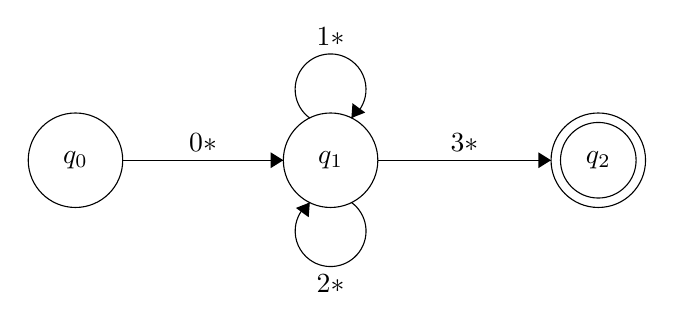
\begin{tikzpicture}[scale=0.2]
\tikzstyle{every node}+=[inner sep=0pt]
\draw [black] (16.3,-25.1) circle (3);
\draw (16.3,-25.1) node {$q_0$};
\draw [black] (32.5,-25.1) circle (3);
\draw (32.5,-25.1) node {$q_1$};
\draw [black] (49.5,-25.1) circle (3);
\draw (49.5,-25.1) node {$q_2$};
\draw [black] (49.5,-25.1) circle (2.4);
\draw [black] (19.3,-25.1) -- (29.5,-25.1);
\fill [black] (29.5,-25.1) -- (28.7,-24.6) -- (28.7,-25.6);
\draw (24.4,-24.6) node [above] {$0*$};
\draw [black] (35.5,-25.1) -- (46.5,-25.1);
\fill [black] (46.5,-25.1) -- (45.7,-24.6) -- (45.7,-25.6);
\draw (41,-24.6) node [above] {$3*$};
\draw [black] (33.823,-27.78) arc (54:-234:2.25);
\draw (32.5,-32.35) node [below] {$2*$};
\fill [black] (31.18,-27.78) -- (30.3,-28.13) -- (31.11,-28.72);
\draw [black] (31.177,-22.42) arc (234:-54:2.25);
\draw (32.5,-17.85) node [above] {$1*$};
\fill [black] (33.82,-22.42) -- (34.7,-22.07) -- (33.89,-21.48);
\end{tikzpicture}
\end{center}
\begin{align}
    0* &= \epsilon, \epsilon\rightarrow \$\\
    1* &= d,\epsilon\rightarrow\epsilon \,|\, c, x\rightarrow\epsilon \,|\,
    b, x\rightarrow\epsilon \,|\, a,\epsilon\rightarrow x \\
    2* &= b,\epsilon\rightarrow y \,|\, c,\epsilon\rightarrow y \,|\, 
    a, y\rightarrow\epsilon \\
    3* &= \epsilon,\$\rightarrow\epsilon
\end{align}
\line(1,0){343px}

\item
Give the 6-tuple $(Q,\sum, \Gamma, \delta, q_0, F)$ for your PDA from a) \\
You do \textbf{not} need to provide the transition function $\delta$.

\vspace{5px}\textbf{Solution ::}
\begin{align*}
    Q &= \{q_0, q_1, q_2\} \\
    \sum &= \{a, b, c, d\} \\
    \Gamma &= \{x, y\} \\
    q_0 &= q_0 \\
    F &= \{q_2\}
\end{align*}

\end{enumerate}
\end{document}